\documentclass{article}
\title{Proposal: Influence Modeling Through Tensor Decomposition}
\author{Robert Lowe}

\usepackage{csquotes}
\usepackage{epigraph}
\usepackage{cite}
\usepackage[]{algorithm2e}
\usepackage{subfig}
\usepackage{graphicx}

%some custom tensor commands
\newcommand{\tens}[1]{\mathcal{#1}}
\newcommand{\ntens}[1]{\hat{\tens{#1}}}

\begin{document}
\maketitle

\section{Introduction}
No document is ever created in a vacuum.  In fact, if a document were
to be created without reference to others it would probably be judged
to be untrustworthy.  This is especially true in the realm of
academic literature where knowledge of source material is absolutely
required to evaluate and study professional work. 

The presently proposed work seeks to study this problem through
a novel technique based on tensor analysis.  The goal is to ascribe
influence to the several documents in a corpus of cited and citing
documents. A secondary goal of the present work is to model the flow
of information from cited to citing papers in such a way that the
topics can be interpreted by intuitively.

\subsection{Impact Metrics}
The metrics used to measure the performance of an academic author are
typically based on citation counts.  Sometimes this metric is based on
the overall citation rate of journals in which publications appear or
they are based on per-paper citations.  As has been noted by several
authors, such as Adler et. al~\cite{adler2009}, these metrics are
often misinterpreted or abused.  For example, Adler cites the
disparity between the rate of publication of biologists and
mathematicians as an instance in which entire disciplines are given
disparaging grades relative to another. Adler also indicates that
merely counting citations may not be an entirely accurate way to gage
influence exerted by a paper on the literature of a field.  Even where
simple citation counts are employed, the time-delay in actual impact
in fields like mathematics make this type of metric unreliable.  Adler
concludes with a survey of common metrics and how they can be used and
misused.

Building on this notion of accuracy, the present work proposes an
approach which looks beyond the simple presence or absence of
citations.  By analyzing the texts of citing and cited documents, the
goal is to build a model which will indicate the strength of influence
exerted by a given paper or collection of papers.  In addition, the
proposed analysis techniques seeks to provide a method by which the
contributions of the author of a citing document can be evaluated.
This is allows the model to evaluate the original impact of an author,
that is to gauge how much original thought an author contributes to
the overall corpus of documents. 

\subsection{Proposed Influence Model}
The proposed model of influence is based on two parts.  First, the
present work will model documents as tensors which model the text of
both citing and cited documents. These tensors will the be decomposed
into rank 1 components which will then be compared for similarity.
The similarities between factors of cited documents and corresponding
factors of the citing document is used to assign weights to each
factor, and by extension to the document comprised of these factors.
These weights comprise the second part of the model where influence of
cited documents is used to explain the composition of the citing
document.  The residuals of this model are interpreted as the citing
author's original contribution to the citing document. The proposed
model is summarized in equation (\ref{eq:model}). 

\begin{equation}
    \label{eq:model}
    C = \sum w_id_i + w_a A
\end{equation}

Here, $C$ is the tensor representation of the citing document.
Individual cited documents are broken up into a set of factors with
each element denoted as $d_i$ which are assigned weights $w_i$.  Finally,
the tensor representing author contribution $A$ is assigned weight
$w_a$.  

\subsection{Related Work}
Text-based influence modelling is still a fairly sparse field of
study.  The present work is, however, heavily influenced by a few
recent works.

First, as has already been noted, Adler et. Al \cite{addler2009}
outlines the need for robust statistics for modelling the actual
influence of an author.  While they do not provide any influence
metrics in the paper, they do propose that such a system should be
adaptable to the fields and corpora in which it is employed.

Another work of note is Dietz et. Al's 2007 paper \cite{dietz2007} which uses
Latent Dirichlet Analysis \cite{blei2003} to provide weights to
a directed graph of topic flow.  Dietz's approach requires
a pre-existing topic model and uses tokenized documents to in
conjunction with LDA to provide influence weights.  The present work
seeks to extract topic models as it models influence, thus requiring
less preprocessing and manual work.

The notion of frequency counting used in the current work was inspired
by El-Arini et Al's 2011 paper\cite{el-arini2011}.  In this work,
influence is modelled by keyword counting.  Again, this requires prior
knowledge of the keywords to be modelled.  El-Arini makes the
assumption that source documents contain keywords in higher
concentrations and uses this to assign influence weights to documents.
One interesting aspect of El-Arini's work is that it attempts to make
a document recommendation system which, given a set of documents and
a set of keywords, can make a set of recommended papers for
a researcher.  El-Arini's work could possibly be improved upon by
using a technique such as the one proposed here to serve as its
influence model.

\section{Approach}
\subsection{Tensors and Decomposition}
The term {\em tensor} carries several different definitions depending
on the field in which it is used.  For the purposes of the present
work, the term {\em tensor} will refer to a multi-dimensional array.
The objective of the tensor models constructed in this approach is to
decompose the tensor into explanatory factors.  Many methods for this
decomposition exist, but the most commonly applied decomposition is
the parallel factors (PARAFAC) decomposition first proposed by by
Harshman in 1970 \cite{harshman1970}.  In PARAFAC, a tensor is
decomposed into a set of factors consisting of rank 1 tensors.  The
decomposition is carried out to satisfy the following equation:

\begin{equation}
    \label{eq:parafac}
    T = \displaystyle\sum_{i=1}^{r} F_i + E
\end{equation}

where $F$ is the set of $r$ rank-1 tensors and $E$ is the error
residual of the model.  Naturally, the ALS algorithm seeks to minimize
the size of $E$.  It is also often convenient to express the factor
tensors in the form of vectors of each component such that the outer
product of these vectors forms the factor.  For instance,
a PARAFAC decomposition of a 3-way tensor can be written as:
\begin{equation}
    \label{eq:parafac-comp}
    T = \displaystyle\sum_{i=1}^{r} A_i \circ B_i \circ C_i + E
\end{equation}

A final common decomposition technique is to normalize the matrices
of the factors giving the final model's representation of:
\begin{equation}
    \label{eq:parafac-lambda}
    T = \displaystyle\sum_{i=1}^{r} \lambda_i A_i \circ B_i \circ C_i
    + E
\end{equation}

Here, the set $\lambda$ indicates the strength of the influence of
each explanatory factor, and so it is often helpful to list factors
such that $\lambda_1 \geq \lambda_2 \geq \ldots \lambda_r$.

PARAFAC is a constrained instance of the Tucker decomposition model,
which in turn is a further constrained principle component analysis
(PCA) deconstruction \cite{bro1997}.  Where a PARAFAC model fits, the
other models will fit as well or better.  However, PARAFAC carries
with it several advantages.  First, it is relatively easy to compute
using alternating least squares regression.  Second, it is unique
under rotation given a sufficiently large number of sought factors
\cite{harshman1970}.  But, perhaps most importantly, PARAFAC
decompositions typically can be interpreted
intuitively~\cite{bro1997}.  

\subsection{Document Model}
In the proposed approach, documents are modeled by using terms along
the dimensions of the tensor.  The vocabulary of the corpus is
represented as words in a sequence $vocab$. 
The document is then divided into
$n$-grams, where $n$ is the number of dimensions of the array.  For
example, a document split into 3-grams would be represented using
a 3 dimensional tensor.  The values of the resultant document tensor
$T$, at index $ijk$ would be the number of occurrences of the 3 word
phrase associated with the sequence of words $ijk$. The total
dimensions of the tensor under this 3-gram scheme would be given 
This allows the approach to be tuned to phrases of any length.  

Naturally, the tensors for even a modest corpus are quite large and
very sparse.  The tensors count the number of occurrences of every
permutation of the vocabulary of length $n$, the vast majority of
which correspond to nonsensical phrases.  Also, the use of the corpus
vocabulary in the indexing of the tensor further increases the
sparsity of the resultant document tensors.

The production of the document model is a two stage process.  First
the corpus is pre-processed according to algorithm \ref{algcorp}.
This is a simple filtering process which leaves only words in the
documents.  (Further development may provide more sophisticated
filtering at this stage.)  After corpus preprocessing is finished,
each document is then modeled as a tensor according to algorithm
\ref{algdoc}.  The result is a collection of tensors, one for each
document, which contains the count of all possible $n$ word phrases.

\begin{algorithm}
\caption{Prepare Corpus}
\label{algcorp}
    Remove Numbers\;
    Remove Punctuation\;
    $wl \leftarrow $ split all documents by spaces\;
    $vocab \leftarrow \emptyset$\;
    \For{$w$ in $wl$} {
        \If{$w \notin vocab$}{
            $vocab$.append($w$)\;
        }
    }
\end{algorithm}


\begin{algorithm}
\caption{Document Tensor Construction}
\label{algdoc}
    $T \leftarrow$ 0 tensor with dimension $|vocab| \times |vocab| \times \ldots
    |vocab|$\;
    $phrase \leftarrow \emptyset$ \;
    \For{$w$ in $d$}{
        $phrase$.append($w$)\;
        \If{$|phrase| = n$}{
            $idx \leftarrow \emptyset$ \;
            \For{$p$ in $phrase$}{
                $i \leftarrow vocab.\mathrm{find}(p)$\;
                $idx.\mathrm{append}(i)$\;
            }
            $T[idx] \leftarrow T[idx] + 1$\;
        }
    }
\end{algorithm}


\subsection{Influence Model}
Having modeled the corpus of documents, all that remains to complete
the model is assign contribution weights to each of the elements in
cited documents as shown in equation (\ref{eq:model}).   This process
begins with decomposing the factors in the citing document $C$ into
the factors $F$ using PARAFAC decomposition.  The components of all
citing documents are then decomposed into the factors $D$, also by
PARAFAC decomposition. Because the data represents counts of phrases,
and is therefore non-negative in nature, a non-negativity constraint
is applied to the decomposition of the documents. Furthermore, each
factor is normalizes as in equation (\ref{eq:parafac-lambda}).

One natural question that arises at this stage is how many factors are
used for each decomposition. This problem is certainly an open area of
research as uniqueness of the solution is only guaranteed when the
number of factors is greater than or equal to the rank of the tensor
being decomposed \cite{harshman1970}.  However, the determination of
the rank of a Tensor is an np-complete problem~\cite{haastad1990}!  To
circumvent this, several metrics can be employed.  Outside knowledge
could be used to determine the correct number of tensors, however
given the present problem no such external knowledge is readily
available.  A more data-based approach is used instead.  The metric
presently used is the core-consistency or CORCONDIA metric proposed by
Rasmus Bro in 2003 \cite{bro2003}.  The core consistency model divides
out each factor in a given tensor and then checks the distance of that
tensor from a superdiagonal tensor.  Completely consistent models have
a CORCONDIA of 100\%, where significant deviation indicates the model
is a poor fit for the given data.  The method employed here is to
decompose each document into different numbers of factors until the
CORCONDIA score drops significantly.  The number of factors just
before the decrease is then selected as this is likely to be greater
than the rank of the tensor, and will certainly provide a good fit to
the data.

Once the number of factors for each document has been determined, the
construction of the model continues with the procedure outlined in
algorithm \ref{alginfluence}.  

\begin{algorithm}
    \caption{Citing Factor Weight Assignment}
    \label{alginfluence}
    $D \leftarrow$ PARAFAC decompositions of cited documents\;
    $F \leftarrow$ PARAFAC decomposition of citing document\;
    $\lambda_d \leftarrow $ Norms of Factors in $D$ (see equation
    (\ref{eq:parafac-lambda})\;
    $\lambda_f \leftarrow $ Norms of Factors in $F$\;
    Normalize $D$ using $\lambda_d$\;
    Normalize $F$ using $\lambda_f$\;
    $w \leftarrow $ matrix of dimension $|D| \times |F|$\;
    \For{$i$ = 1 to $|D|$} {
        \For{$j$ = 1 to $|F|$} {
            $w[i,j] \leftarrow \mathrm{similarity(D[i], F[i)}$;
        }
    }
\end{algorithm}

The output of algorithm \ref{alginfluence} is a matrix with similarity
scores for each of the factors. The columns represent the citing
document factors, with each row showing the similarity measure for
each candidate cited factor.  The algorithm leaves out an explicit
definition of the similarity metric as this is a matter to be explored
in the proposed research. For now, a simple metric is employed as
a proof of concept.  

The selection of the similarity metric should be made such that its
output is between 0 and 1, and it should roughly correspond to the
proportion of variability of the factor in $F$ which can be explained
by $D$.  Because the contents of $F$ and $D$ are all proportions,
given the normalization carried out in the PARAFAC process, one simple
measure which satisfies this constraint is root mean square deviation
between the factors.  This is easy to compute and test, and given
non-negative factors between 0 and 1 it will always yield results in
that range.  However, this makes a broad range of assumptions, not
least is a linear relationship between the transfer of topics from the
source documents to citing document.  This part of the model should
therefore be regarded as a place holder until further study is carried
out.  Also, RMSD is a measure of deviation, so really what is needed
for this place-holder metric is $1-\mathrm{RMSD}(d_i, f_i$, and this
is what is used in the example application in the next section.

Another open question for the present research is how to combine these
weights.  The resultant weight matrix could, of course, be normalized
and treated as the weight distribution for the influence model,
however this leads to a break down of the goals outlined in the first
section.  Namely, there would be no residuals.  Such a normalization
would imply that all of the factors of the citing document were fully
explained by the factors in the cited documents.  Stated another way,
such an assumption would be equivalent to assuming that the citing
author has contributed nothing!  For the the present example problem,
the assumption that is made is that each factor in the citing document
can only be described by one of the cited factors (though any one
citing factor may be able to explain any number of citing factors).
This assumption is, of course, quite dangerous in the general case but
will work for showing the relative merits of this model in this
proposal.  Using this assumption, the model is advanced by selecting
the maximum weighted factor for each column.  The rest of each factor
being treated as a residual.  This temporary algorithm is shown in
algorithm \ref{algselection}.

\begin{algorithm}
    \caption{Temporary Factor Selection}
    \label{algselection}
    $indexes \leftarrow \emptyset$\;
    $weights \leftarrow \emptyset$\;
    \For{$c$ = 1 to $|F|$}{
        $i \leftarrow $ index of maximum weight in column $c$ of $w$\;
        $indexes.\mathrm{append}(i)$\;
        $weights.\mathrm{append}(w[i,c])$\;
    }
\end{algorithm}

The results of algorithm \ref{algselection} are the
indexes and the weights of the selected factors.  These represent the
proportion of contributions for each factor.  If every factor had
a uniform explanatory effect on the citing document, the model would
be complete at this step.  Of course, this almost never happens.  The
normalizing scalars $\lambda$ indicate the strength of each factor in
$f$.  To arrive at the overall weights and proportions for each
contributing factor requires that the weights be scaled by their
overall proportion to the citing document.  This final modification of
the weights is shown in algorithm \ref{algadjust}.

\begin{algorithm}
    \label{algadjust}
    \caption{Proportional Weight Adjustment}
    $s \leftarrow \sum \lambda_f$\;
    \For{i = 1 to |w|} {
        $w[i] \leftarrow \lambda_f[i] * w[i] / s$\;
    }
\end{algorithm}

At this stage the author's contribution weight can be computed as
shown in equation (\ref{eq:authorWeight}).  The present method in this
proposal does not, however, provide a clear way to extract the author
contribution tensor.  This is left to the future development of this
work.

\begin{equation}
    \label{eq:authorWeight}
    w_a = 1 - \sum w
\end{equation}

Likewise, the contributions of each document can readily be computed
by summing the weights associated with each citing document.  This
mapping is trivial given the $indexes$ list extracted during algorithm
\ref{algselection}. 

\section{Example Problem}
Testing the proposed algorithm is tricky.  As is the case with most
text modelling, simply reading the texts in question give little
insight into appropriate numerical weightings of the contribution.  In
order to alleviate this problem, and produce a test data set with at
least some element of ground truth knowledge, a simple dataset is
generated from known contributing elements.  Also, present limitations
of available software mandates a data set with a relatively small
vocabulary.

The analysis in this example problem was carried out using Rasmus
Bro's n-way toolkit \cite{andersson2000} for Matlab (though GNU Octave was used as the
actual interpreter.)  This package, though it works with Matlab's
sparse arrays, has a tendency to unfold sparse arrays into dense
arrays.  As such, it has difficulty handling tensors that will not fit
into a computer's memory.  

So then the example problem must be generated with two goals in mind.
First, it must have at lest somewhat knowable proportions.  Second, it
must have a small enough vocabulary so that its tensors and
decompositions will not exceed a few gigabytes in size.

\subsection{Test Set Creation}
The test problem presented here consists of a three document corpus.
The first two documents are taken from the children's stories {\em The
Ant and the Dove}~\cite{aesop} and {\em The Seven
Ravens}~\cite{aesop}.  These documents comprise the cited documents in
the corpus.  A third document, referred to as the "generated"
document, is produced using a software package called
DadaDodo~\cite{dada}.  DadaDodo builds a Markov-Chain based model of
its source material and generates a new document by sampling the
Markov chains for word order probability.  The output of DadaDodo
tends to be at least somewhat grammatically correct, but is generally
nonsense. 

In fact, in this instance, the generated document has a weak plot
which is somewhat of a mixture between the plot of the two stories.
To the extent meaning can be ascribe to the generated story, it is
a rather grisly tale of a young girl who feeds a dwarf to a raven
while her father searches for an ant and a dove.  For instance,
consider the excerpt in figure \ref{fig:gentext}.

\begin{figure}
  \label{fig:gentext}
  \begin{displayquote}
But the glass, she the ring drumstick, of men! 

But a morsel from each of wings and looked at it was true that wish I am
looking for a little chair as he was once a human mouth. 
  \end{displayquote}
  \caption{Excerpt of Generated Text}
\end{figure}

More interesting, of course, is the statistical situation of the
samples.  The first stage of the analysis as show in 
algorithms \ref{algcorp} and \ref{algdoc}, is to generate tensor
representations of the documents.  For the sake of simplicity,
a 3-gram analysis is carried out yielding the statistics shown in
table \ref{tab:docstats}.

\begin{table}
    \label{docstats}
    \begin{tabular}{l|r|r}
    {\bf Document} & {\bf Distinct 3-grams} \\
    \hline
    {\em The Ant and the Dove} & 258 \\
    {\em The Seven Ravens} & 939 \\
    \hline
    {\em Generated Document} & 619\\
    \end{tabular}
    \caption{Document Phrase Statistics}
\end{table}

Because the generated document is generated according to the Markov
assumption, it has the capacity to invent new phrases.  The overall
probabilities are an even mixture of the word order probabilities of
the two documents.  As such, both documents should be more or less
evenly present in the generated document, with some residual left over
for the mixture of the two.  In this example, the generated document
contains $619$ distinct 3-grams, $372$ of which do not appear in the
source material.  Thus the expected contributions for the author and
the documents can be estimated as shown in table \ref{tab:expected}. The
high author contribution is reasonable and desirable given the end
goal of analyzing real-world citing documents.

\begin{table}
    \label{tab:Expected}
    \begin{tabular}{l|r}
    {\bf Document} & {\bf contribution} \\
    \hline
    Ant &  0.2261 \\
    Raven & 0.2261 \\
    $w_a$ & 0.54 \\
    \end{tabular}
    \caption{Expected Contributions}
\end{table}

All three of the documents in the corpus are well represented by
a five factor decomposition. This was discovered by means of repeated
decomposition and observation of the CORCONDIA metric as outlined
previously.  The data are then processed using algorithms
\ref{alginfluence}, \ref{algselection}, and \ref{algadjust}.

\subsection{Results}
The resultant factor statistics are shown in table \ref{tab:results}.  The
performance of the algorithm is pretty much as expected.  However,
observing the graphical representation of all the matched factors show
that most of the matched factors have few features in common with each
other.  This is attributable to the primitive matching method used,
and will require further effort to refine.

\begin{table}
    \label{tab:results}
    \begin{tabular}{l|r|l}
        {\bf Factor 1} & {\bf Explanatory Weight} & {Source}\\
        \hline
        1 & 0.06 & Ant Factor 3\\
        2 & 0.04 & Ant Factor 3\\
        3 & 0.12 & Raven Factor 3\\
        4 & 0.14 & Ant Factor 1\\
        5 & 0.10 & Raven Factor 1\\
    \end{tabular}
    \caption{Factor Results}
\end{table}


Summing these results and calculating the residual yields the document
and author contributions shown in table \ref{tab:docresults}.  These
results match the expected results fairly closely indicating that the
decomposition and matching worked as expected.

\begin{table}
    \label{tab:docresults}
    \begin{tabular}{l|r}
        {\bf Source} & {\bf Contribution} \\
        \hline
        {\em The Ant and the Dove} & 0.24 \\
        {\em The Seven Ravens} & 0.22 \\
        $w_a$ & 0.54
    \end{tabular}
    \caption{Document Contribution Results}
\end{table}

\begin{figure}%
    \centering
    \subfloat{{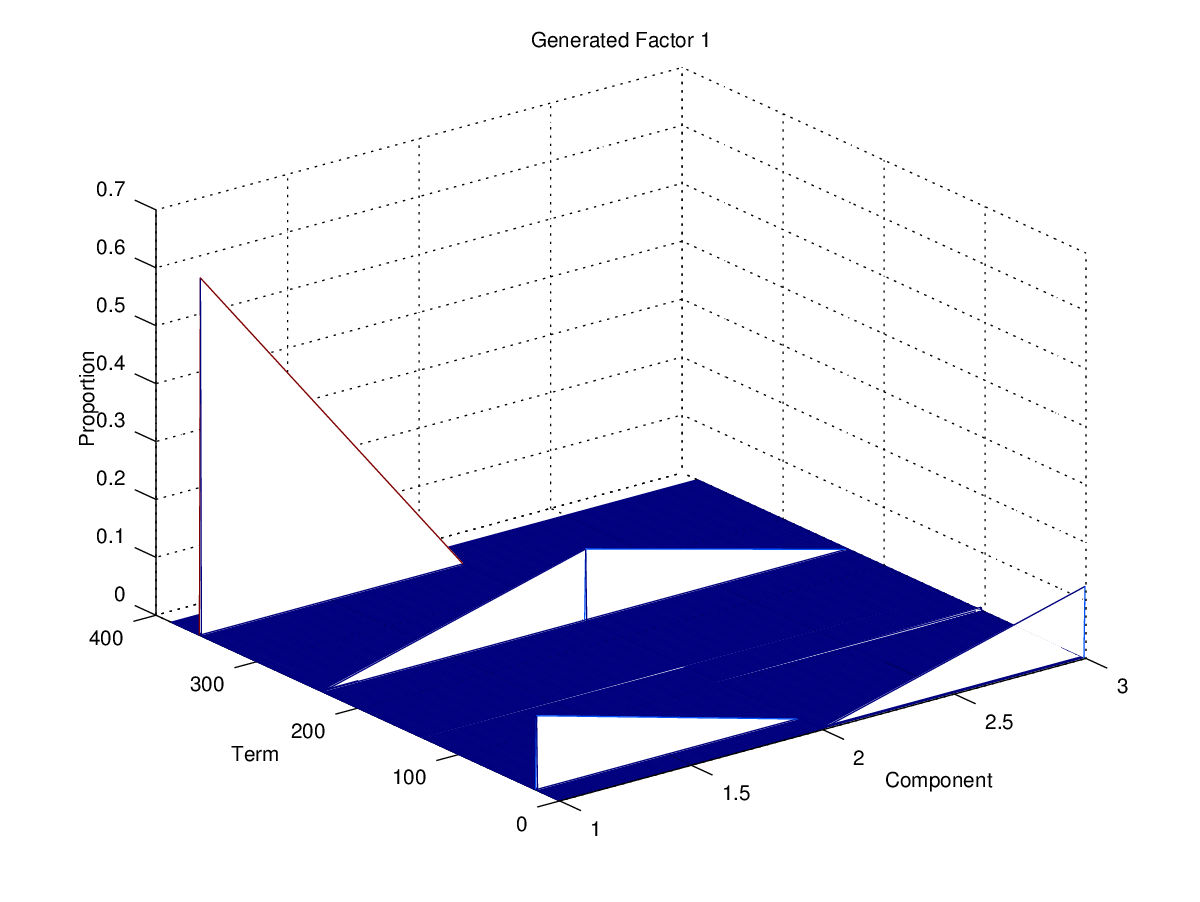
\includegraphics[width=5cm]{plots/gen1} }}%
    \qquad
    \subfloat{{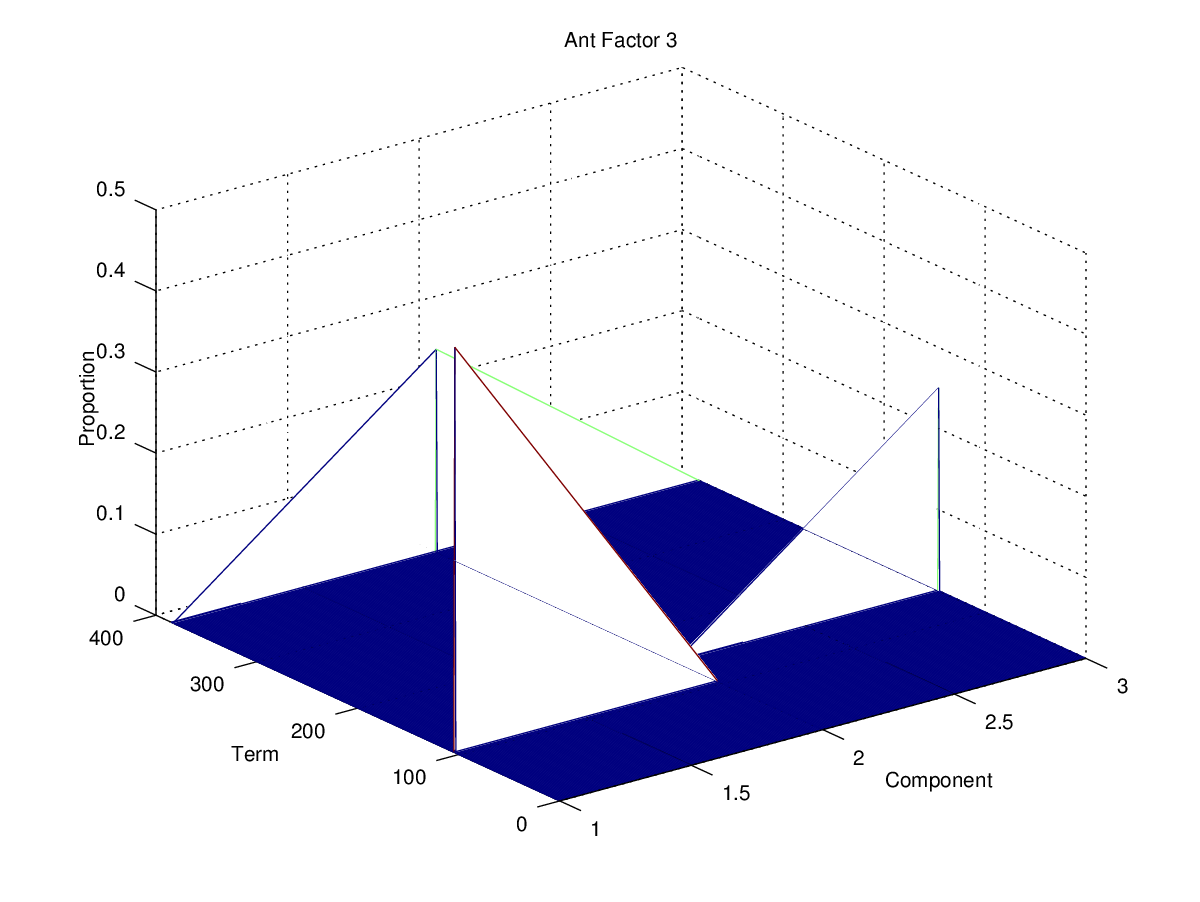
\includegraphics[width=5cm]{plots/ant3}
    }}%
    \caption{Component 1 Match}%
    \label{fig:com1}%
\end{figure}

\begin{figure}%
    \centering
    \subfloat{{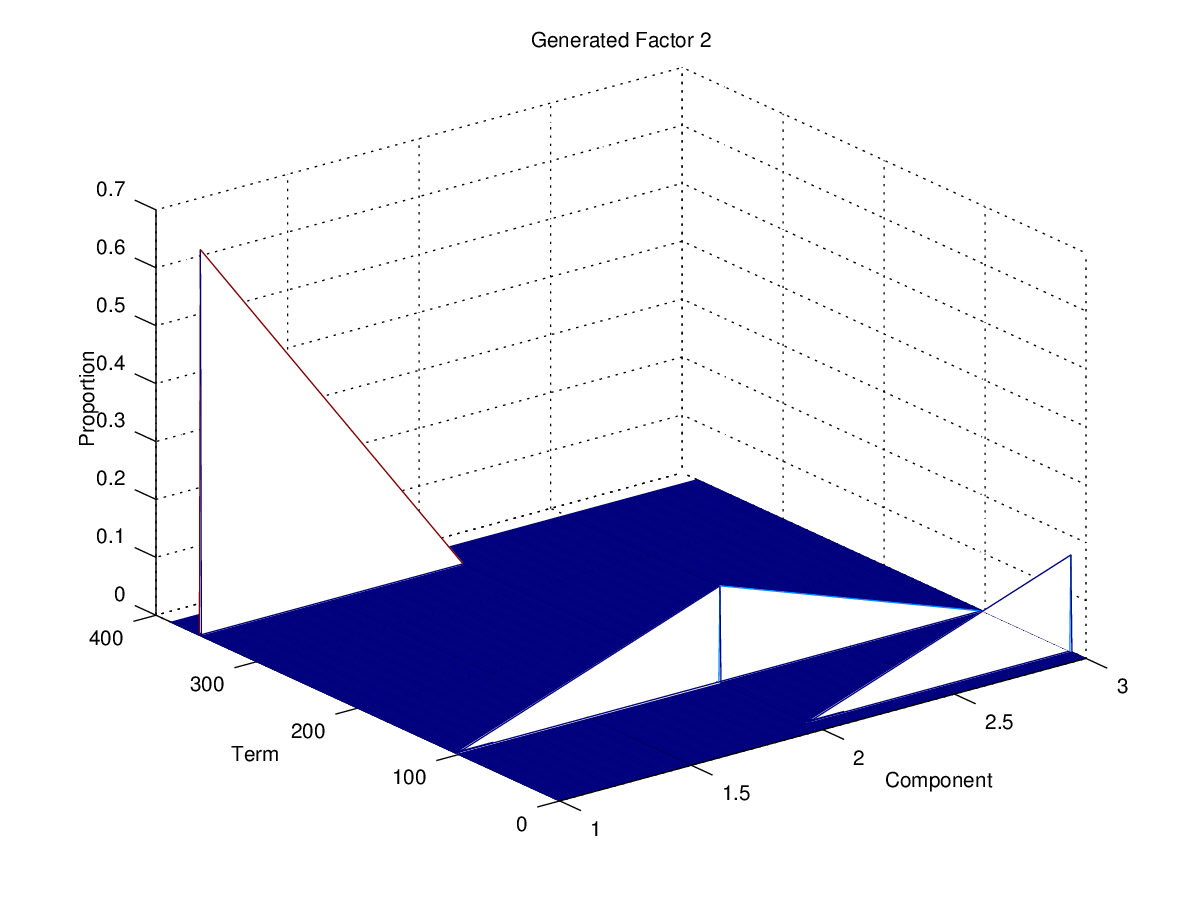
\includegraphics[width=5cm]{plots/gen2} }}%
    \qquad
    \subfloat{{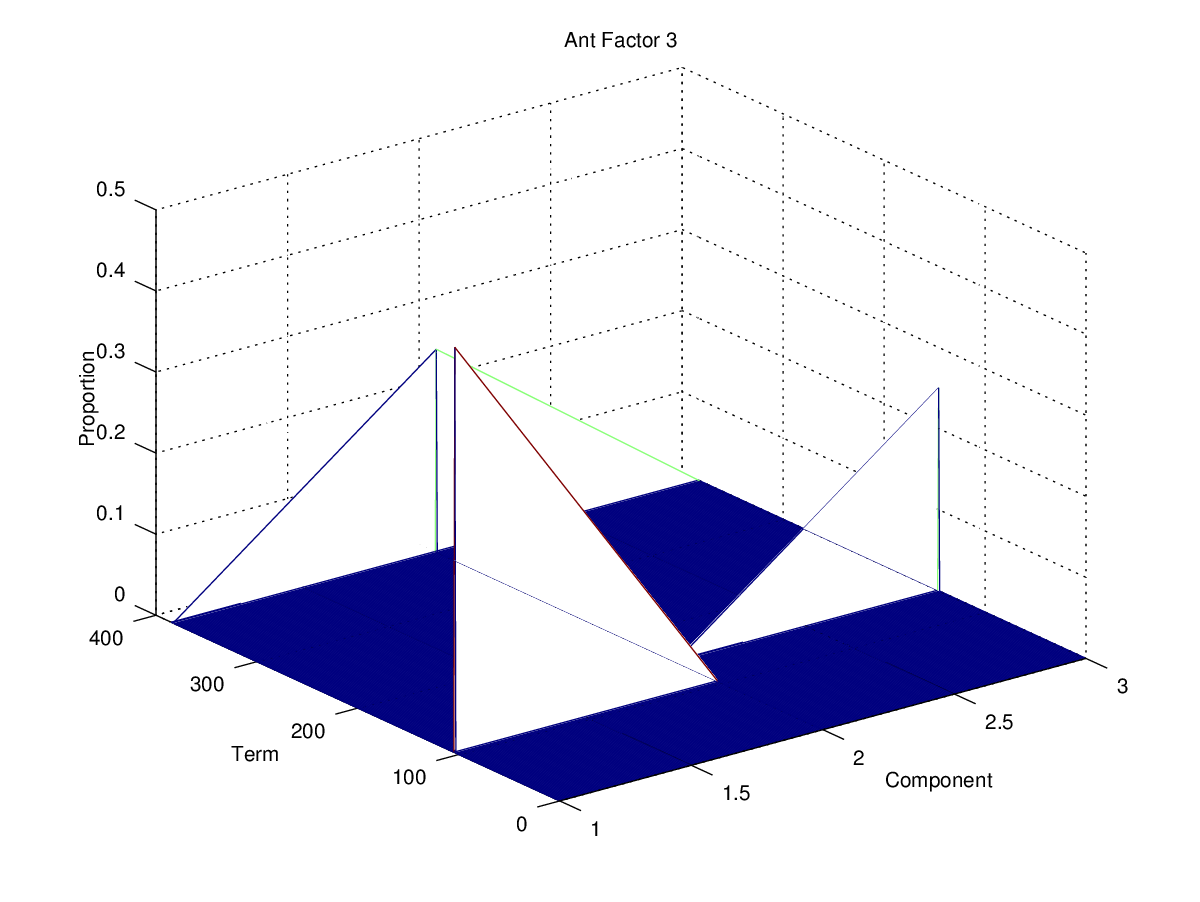
\includegraphics[width=5cm]{plots/ant3}
    }}%
    \caption{Component 2 Match}%
    \label{fig:com2}%
\end{figure}

\begin{figure}%
    \centering
    \subfloat{{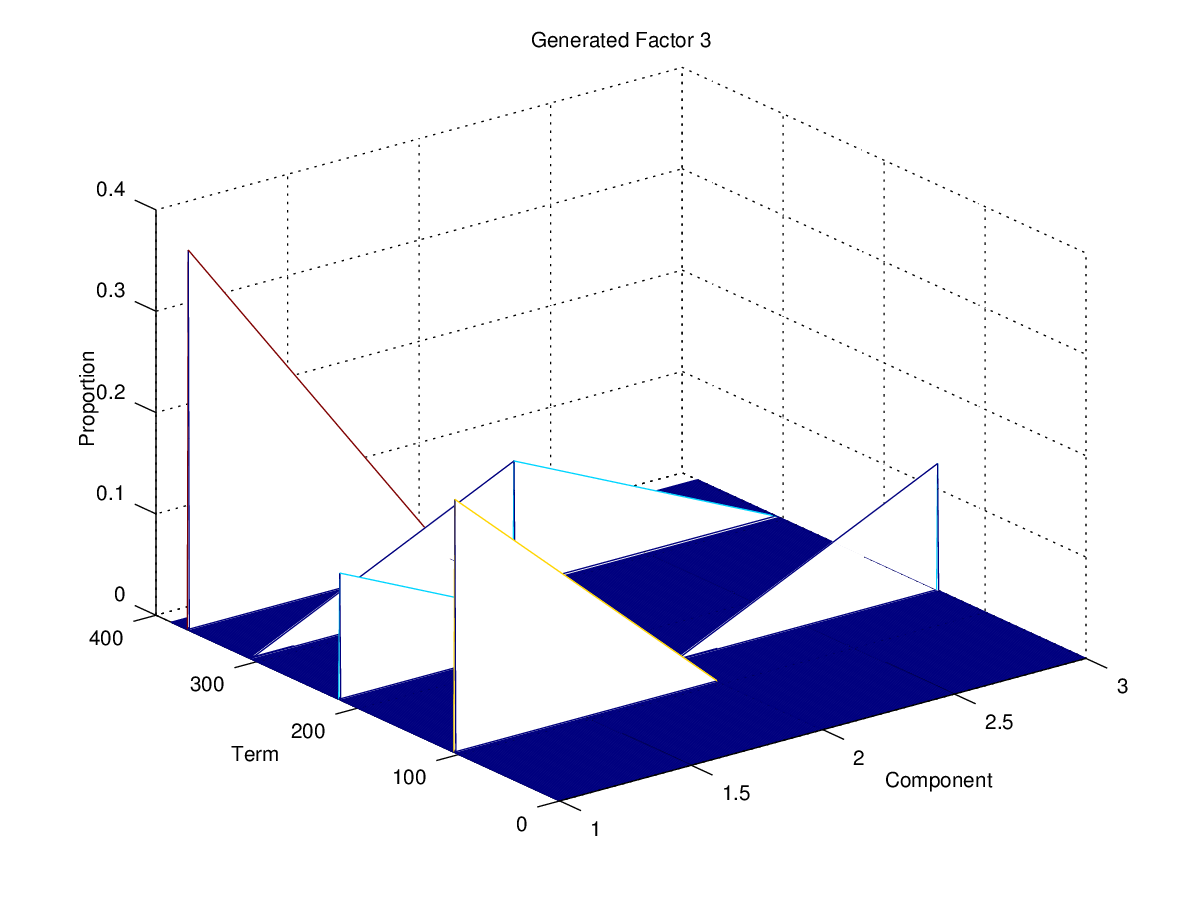
\includegraphics[width=5cm]{plots/gen3} }}%
    \qquad
    \subfloat{{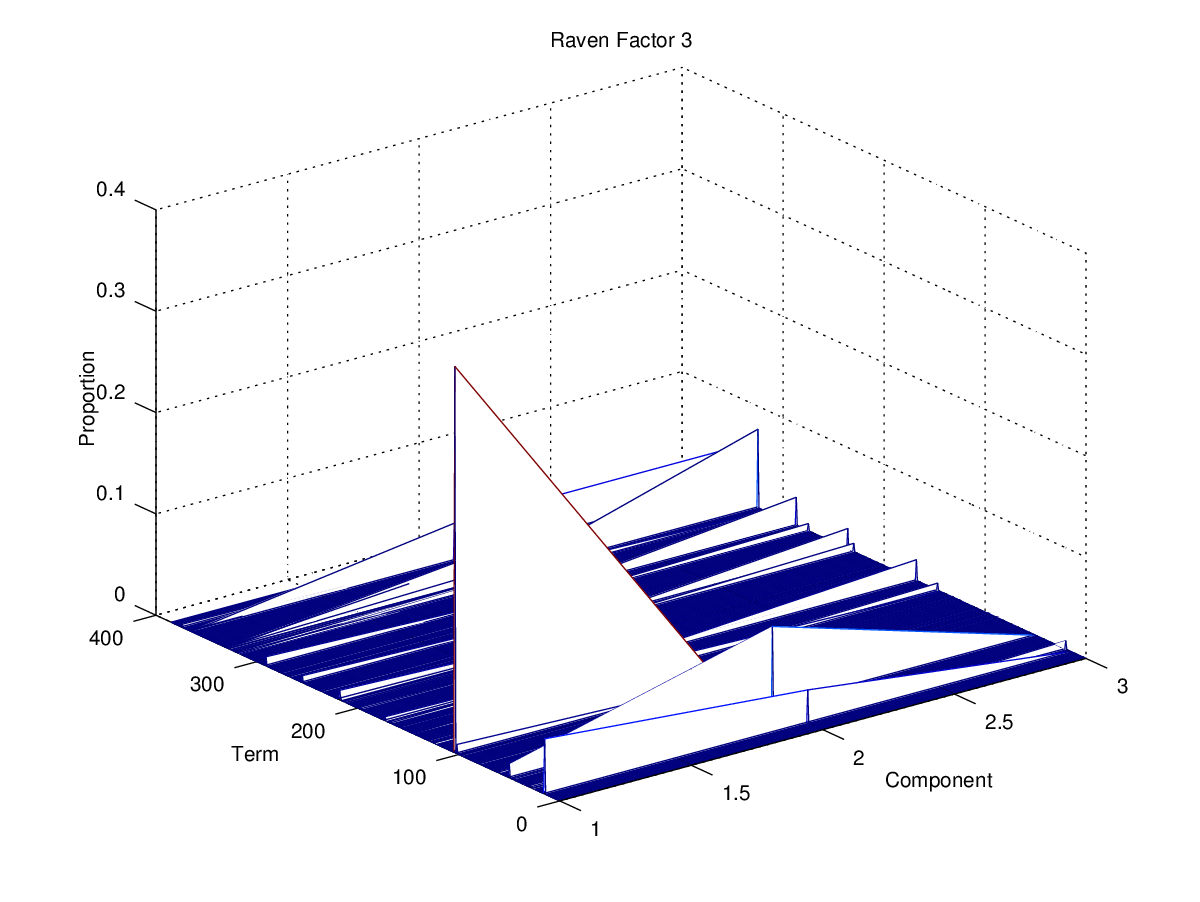
\includegraphics[width=5cm]{plots/rav3}
    }}%
    \caption{Component 3 Match}%
    \label{fig:com3}%
\end{figure}

\begin{figure}%
    \centering
    \subfloat{{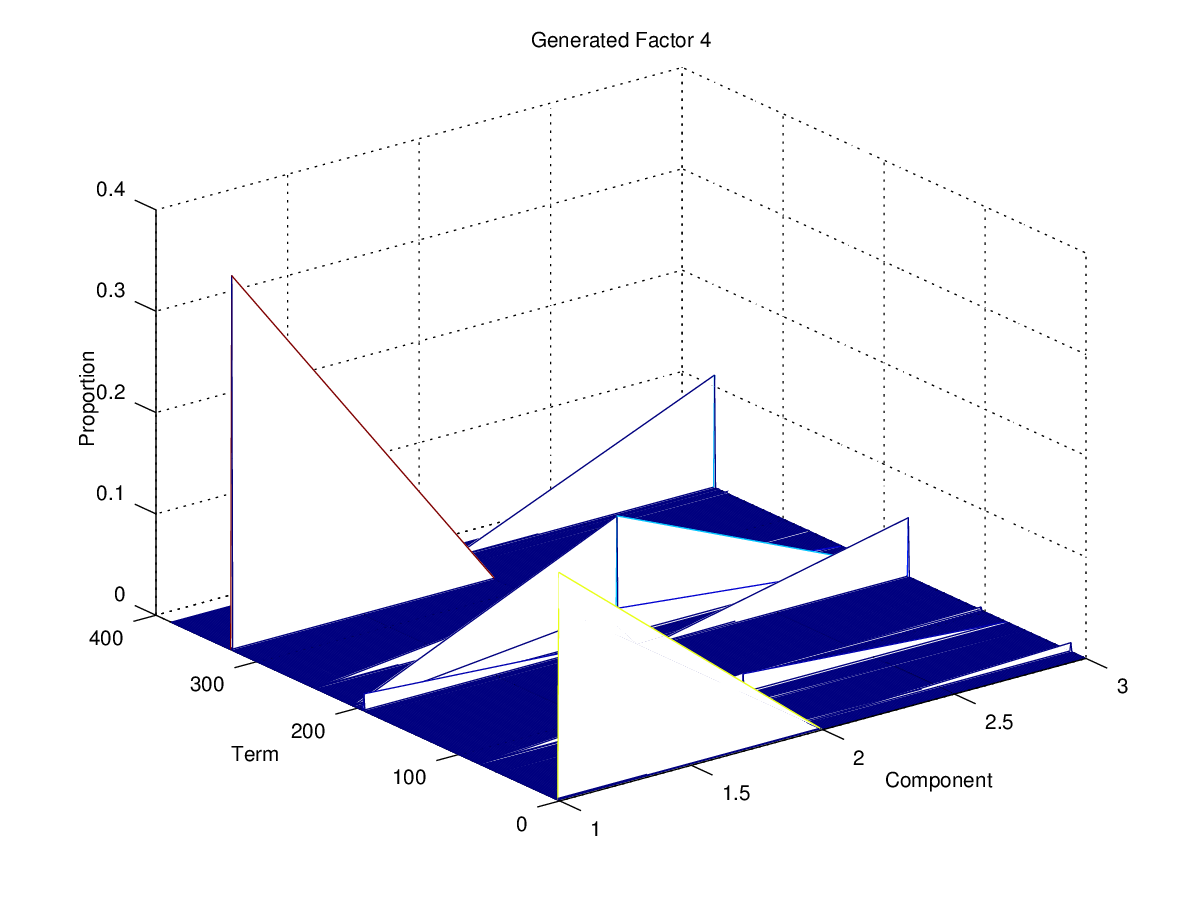
\includegraphics[width=5cm]{plots/gen4} }}%
    \qquad
    \subfloat{{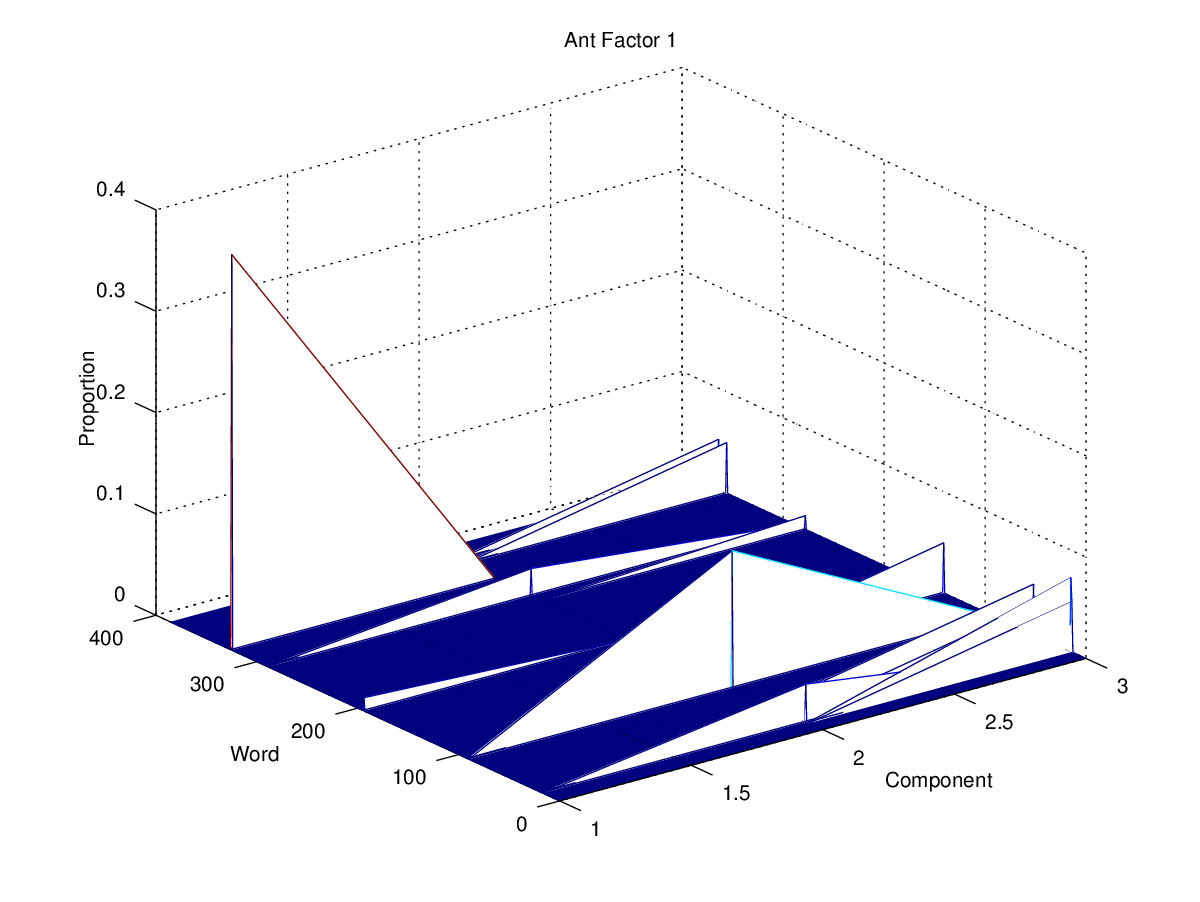
\includegraphics[width=5cm]{plots/ant1}
    }}%
    \caption{Component 4 Match}%
    \label{fig:com4}%
\end{figure}

\begin{figure}%
    \centering
    \subfloat{{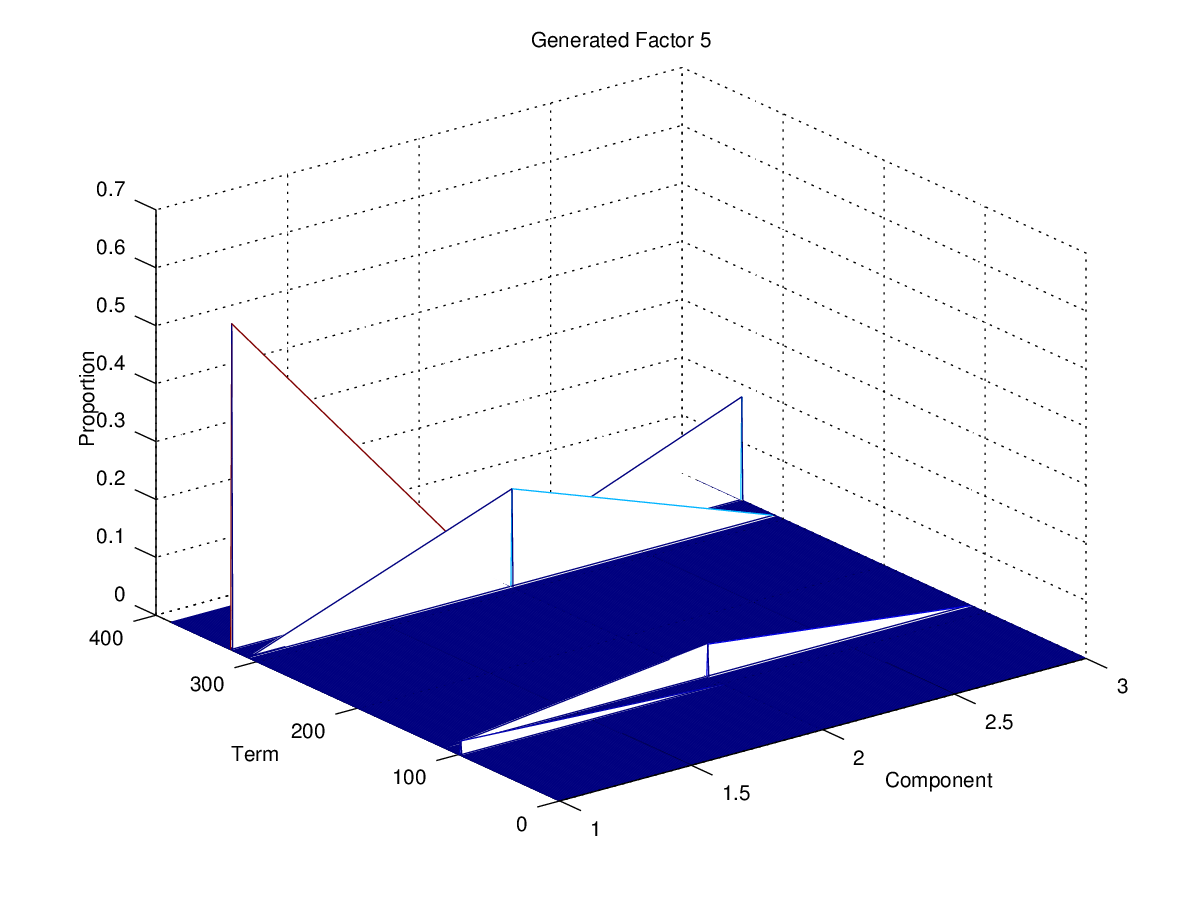
\includegraphics[width=5cm]{plots/gen5} }}%
    \qquad
    \subfloat{{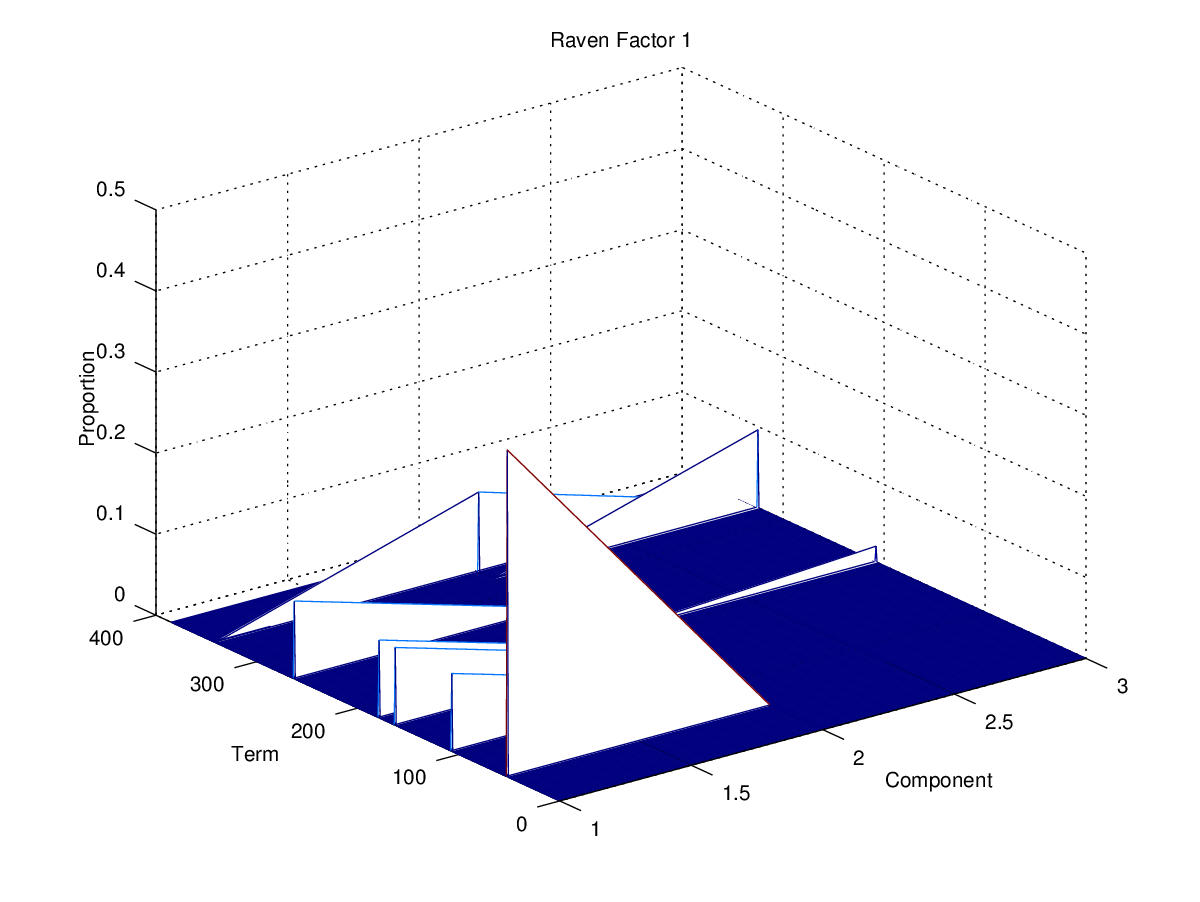
\includegraphics[width=5cm]{plots/rav1}
    }}%
    \caption{Component 5 Match}%
    \label{fig:com5}%
\end{figure}

\section{Proposed Contributions and Further Work}
The preliminary results appear encouraging, and so the proposed work
is to continue development of this influence modelling technique.  The
key contributions of the proposed work are outlined in this section.

\subsection{Influence Model}
The influence model itself warrants further study and analysis.
Particularly, a more sophisticated metric is needed for comparing the
factors of the decomposed tensors.  This will be accomplished through
comparison of the performance of several metrics.

Another related contribution sought by the proposed work is a method
to evaluate the validity of a tensor-based influence model.  This
will, of course, be heavily influenced by the selected method or
methods of modeling factor contributions.

\subsection{Filtering}
This technique, as it stands now, assumes that the originating sources
of all n-grams are contained within the document corpus being
analyzed. This is, of course, not true.  In fact, there will be many
phrases and even groups of phrases common to many different documents
within a corpus.  A filtering technique would be useful to avoid
attribution of these common phrases.

On the other hand, these common phrases may indicate some level of
stylistic influence exerted by an author.  In either case, determining
commonalities among the several documents within the corpus prior to
assigning attribution weights should prove an interesting area of
study and validation of the proposed model.

\subsection{Software}
Another contribution sought is in tensor software creation.  The size
and complexity of the tensors in the present work demand more robust
tensor factoring software.  Current packages cannot handle the very
large sparse tensors present in a real-world application.  As such,
the proposed work will include a tensor library written in C++ which
will be able to handle the task of large sparse tensors.  This
software will be released under some suitable open source license.

\subsection{Additional Applications}
Once a working model is in hand, additional extensions of application
will be tried. Some proposed future directions include:
\begin{itemize}
    \item Topological sorting to determine chronology of documents
    based on influence modelling.
    \item Identification of uncited documents in a corpus which appear
    to have exerted an influence.
    \item Modelling of transitive influence by observing the flow of
    factors through the influence network.
\end{itemize}


\section{Conclusion}
Modelling document influence is an interesting computational problem
with potentially interesting applications.  The present proposal is to
build a solution of this model using tensor decomposition to analyze
the flow of ideas from cited paper to citing paper in a corpus of
scientific literature.  The proposed solution to this problem will
work without prior knowledge of the contents of corpora, and so it
should prove to be a generally useful modelling technique.


\bibliography{sources}{}
\bibliographystyle{plain}

\end{document}
